\section{Sterowanie ekranem}
\label{sec:component-controll-remote-screen} % marker umożliwiający odwolanie z sekcji architektura

\subsection{Wstęp}

Klient to komputer podłączony bezpośrednio do ekranu wyświetlającego obraz. Istotnymi cechami takiego urządzenia są przede wszystkim:
\begin{itemize}
	\item niska cena
	\item wystarczająca moc obliczeniowa do uruchomienia przeglądarki, oraz prostej gry w technologi Flash, lub HTML5
	\item duża dostępność
	\item mały rozmiar
\end{itemize}

Głównym zadaniem klientów jest komunikacja serwerem poprzez sieć Ethernet w celu wyświetlania obrazu na podłączonym do klienta ekranie, oraz możliwość sterowania urządzeniami wejścia (klawiatura, myszka) poprzez udostępniony interfejs w sieci Ethernet.


\subsection{Hardware}

\subsubsection{Architektura procesora}
Jeśli chodzi o wybór architektury procesora wybór był całkiem prosty, za sprawą sporej liczby dostępnych urządzeń dostępnych w tej architekturze (32 bitowa architektura ARM\footnote{Advanced RISC Machine} jest najczęściej stosowaną architekturą w urządzeniach mobilnych\cite{acm}), jak i uzasadnioną ich popularnością. Architektura ARM cechuje cię niskim poborem energii, dużą niezawodnością w systemach wbudowanych, oraz dla praktycznie wszystkich dostępnych na rynku procesorów możliwością instalacji systemu operacyjnego.
Procesory oparte o architekturę ARM przetwarzają instrukcje z wykorzystaniem mechanizmu potokowania. Procesor może wykonywać trzy rodzaje instrukcji:
\begin{itemize}
	\item 32-bitowe ARM
	\item 64-bitowe ARM (Apple A7)
	\item 16-bitowe Thumb (oraz Thumb2)
\end{itemize}

Firma ARM projektuje rdzenie procesorów i sprzedaje je producentom. Producenci z kolei tworzą rozwiązania Soc \footnote{System on Chip} - dodawane są bloku funkcyjne, jednostki wektorowe czy procesory sygnałowe. Istnieje też spora lista firm, które projektują swoje rdzenie wykorzystujące zbiór instrukcji ARM m.in. Apple, XScale, Faraday.

Istotną cechą, którą powinien posiadać procesor ARM jest jednostka MMU\footnote{Memory Managment Unit}. Jest to jednostka odpowiadająca za dostęp do zewnętrznej pamięci, translacje adresu wirtualnego na fizyczne, oraz kontroli uprawnień dostępu do paimęci. Wiele rdzeni ARM nie jest wyposażonych w tą jednostkę, która staje się obligatoryjna podczas gdy chcemy zainstalować system operacyjny Linux na urządzeniu. 


Po wyborze architektury procesora należy wybrać rodzinę procesora. Rodzina Cortex jest kolejną generacją procesorów po ARM7, ARM9, czy ARM11.

\begin{figure}
\begin{center}
	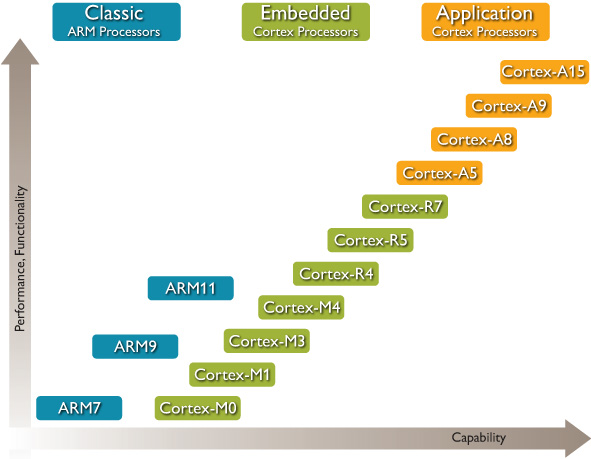
\includegraphics[scale=0.6]{ARM_Comparison}
\end{center}
\caption{Porównanie rodzin architektury ARM}
\label{fig:ARM_Comp}
\end{figure}

Zgodnie z tym co można zauważyć na rysunku~\ref{fig:ARM_Comp} architektura Cortex jest rodziną cechującą się wyższym od swoich poprzednikow współczynnikiem wydajności na cykl zegara i niższym zużyciem energii.

Jak już zostało wspomniane duży wybór komputerów opartych o rdzenie ARM jest spowodowane tym, że wielu producentów produkuje SoC bazując na rdzeniach firmy ARM. I tak na rynku można wyodrębnić 3 główne:
\begin{itemize}
	\item Allwinner (sunxi)
	Przykladowe produkty:
	\begin{itemize}
		\item Hackberry A10
		\item MK802
	\end{itemize}

	Chipy Allwinnera charakteryzują się najniższą ceną, oba przedstawione wyżej modele bazują na rdzeniu Cortex-A8 taktowane zegarem 1GHz, oraz dysponujące 1GB pamięci operacyjnej. Wyposażone są także w procesor graficzny ARM Mali 400
	
	\item Freescale i.MX6 (imx)
	Przykładowe produkty:
	\begin{itemize}
		\item MarS
		\item IMX53QSB
	\end{itemize}
	Produkty Freescale nie posiadają najlepszego stosunku możliwości do ceny przez co też prawdopodobnie nie zyskały sporej popularności w internecie.
	\item TI OMAP3/4
	Przykładowe produkty:
		\begin{itemize}
			\item Beaglebone Black
			\item Panda Board
		\end{itemize}
	Ta rodzina zyskała największą popularność. OMAP3 wyposażone jest w zmiennoprzecinkową jednostkę oraz zestaw instrukcji wktorowych NEON. Główną cechą jest dużo wydajność operacji przy zachowaniu prostoty ich programowania.
\end{itemize}



\subsection{System operacyjny Linux}

Nie dysponując zbyt dużą mocą obliczeniową, małą pamięcią operacyjną, oraz niewielką przestrzenią dyskową należy dobrze dobrać, oraz skonfigurować system operacyjny. Do tego celu wybrano dystrybucje Linuksa - Debian. Cechuje się ona przede wszystkim wysoką stabilnością (bardzo często wybierana jako system serwerowy), oraz sporą społecznością użytkowników co przekłada się na mnogość dostępnych pakietów przygotowanych specjalnie dla tej wersji systemu Linux. Wreszcie system Debian jest wysoce konfigurowalny - oparty o jądro Linux, daje użytkownikowi możliwość zbudowania systemu od podstaw.

Do zbudowania systemu Linux opartego o architekturę ARM posłużono się istniejącą instalacją Debian na komputerze PC. 

\subsubsection{Przygotowanie bazowej wersji systemu}

\begin{figure}
\begin{center}
    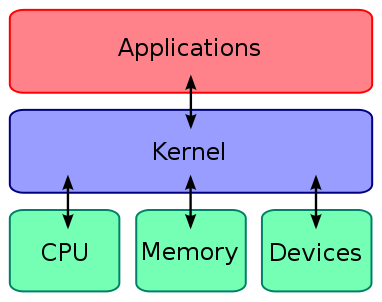
\includegraphics[scale=1]{kernel}
\end{center}
\caption{Działanie jądra systemu Linux}
\label{fig:kernel}
\end{figure}

Jądro systemu Linux jest centralnym miejscem systemu operacyjnego. Jak zaprezentowano na rysunku ~\ref{fig:kernel} jest najniższą warstwą systemu operacyjnego odpowiadająca za komunikację z procesorem, pamięcią, czy urządzeniami zewnętrznymi. Kernel m.in. przydziela odpowiednią ilość pamięci operacyjnej dla każdej aplikacji, obsługuje komunikaty, obsługuje komunikacje między procesorową.

Pierwotnym twórcą jądra Linux jest duńczyk Linus Torvalds, natomiast obecnie jądro systemu Linux jest rozwijane przez programistów z całego świata. Jego aktualną wersje można pobrać z repozytorium Linusa Torvaldsa.

Instalując dystrybucję linuksa na komputerze PC zwykle nie ma to sensu by kompilować jądro samemu. Większość dystrybucji udostępnia gotowy obraz, który zawiera podstawowe programy i usługi niezbędne dla podstawowego systemu operacyjnego. W przypadku systemu wbudowanego wygląda to nieco inaczej. Nie ma jednego gotowego obrazu pasującego do wszystkich jednoukładowych komputerów.


Niezbędnymi narzędziami do zainstalowania systemu są:
\begin{itemize}
	\item {\lstinline|gcc-x-arm-linux-gnueabi|}  - kompilator dla architektury ARM. Fraza eabi, znajdująca się na końcu nazwy tego pakietu to pewien standard opracowany przez firmę ARM. ABI  \footnote{ang. \emph{Application Binary Interface}} jest to zestaw reguł i ustawień kompilacji, które decydują o tym jak dany program współpracuje z innymi bibliotekami, czy aplikacjami. Programy skompilowane przy pomocy kompilatora używającego standardu EABI są przenośne pomiędzy systemami operacyjnymi (jedyną barierą są biblioteki z którymi współpracuje dany program).
	\item {\lstinline|build-essential|} - jak sama nazwa wskazuje jest to zbiór pakietów niezbędnych do budowania oprogramowania. Zależnościami tego pakietu to m.in. g++, libc, czy make.
	\item {\lstinline|git|} - system kontroli wersji
	\item {\lstinline|u-boot-tools|} - zestaw narzędzi do bootloadera, który zostanie opisany w dalszej częsci pracy.
\end{itemize}

Następnym krokiem jest ściągnięcie kodu źródłowego jądra, z racji tego, że architektura ARM Allwinner sun4i nie jest oficjalnie wspierana przez repozytorium Linusa Torvaldsa, posłużono się repozytorium wywodzącym się z niego przystosowanym do potrzeb tej architektury.

Aktualną wersję jądra można pobrać za pomocą polecenia: \lstinline|git clone https://github.com/linux-sunxi/linux-sunxi|. Za pomocą polecenie należy się przełączyć na odpowiednią gałąż oprogramowania \lstinline|git checkout sunxi-3.4|. By skompilować jądra należy wykonać polecenia:

\begin{lstlisting}
make ARCH=arm CROSS_COMPILE=arm-linux-gnueabi- sun4i_defconfig
make ARCH=arm CROSS_COMPILE=arm-linux-gnueabi- -j16 uImage modules
make ARCH=arm CROSS_COMPILE=arm-linux-gnueabi- INSTALL_MOD_PATH=output modules_install
\end{lstlisting}

W pierwszej linii generowana jest standardowa konfiguracja jądra dla danej platformy. Parametr \lstinline|ARCH=arm| określa architekturę jądra. Parametr \lstinline|CROSS_COMPILE=arm-linux-gnueabi-| określa przedrostek cross kompilatora, używany przy budowaniu i przy instalacji (czyli cross kompilator dla polecenia w liniach 1-3 to arm-linux-gnueabi-gcc).
\\
W linie drugiej budowane są moduły jądra, oraz plik z jądrem, oraz następnie dodawana do niego jest suma kontrolna, oraz informacje wymagane przez bootloader. Parametr j16 jest parametrem programu \lstinline|make| określającym ile jednocześnie zadań może być uruchamianych, przez zadanie w przypadku programu \lstinline|make| rozumiane jest rozwiązanie jednej zależności. Program make za pomocą grafu zależności określa kolejność wykonywanych zadań.
\\
Komenda z linii trzeciej instaluje moduły w zadanej lokacji.




System debian zostanie zainstalowany na karcie SDHC \footnote{ang. \em{Secure Digital High Capacity}}, po czym zostanie uruchomiony na urządzeniu Rickomagic MK802 II. Komputer ten opiera się o architekturę ARM Cortex-A8, bazuję na chipie firmy AllWinner sun4i.
\\
\\
	\begin{table}[t]
		\centering
		\caption{SD Card Layout}
		\label{tab:sd-layout}
	\begin{tabular}{|c|c|c|}
	\hline
	\textbf{Start} & \textbf{size} & \textbf{usage} \\ 
	\hline
	0 & 8KB & Nieużywane, dostępne do układu partycji \\
	\hline
	8 & 24KB & SPL \footnote{ang. emph{Secondary Program Loader}} \\
	\hline
	32 & 512KB & u-boot \\
	\hline
	544 & 128KB & Środowisko \\
	\hline
	672 & 352KB & Zarezerwowana \\
	\hline
	1024 & - & Dostępne dla partycji \\
	\hline
	
	
\end{tabular}
\end{table}

W tabeli ~\ref{tab:sd-layout} przedstawiono rozkład pamięci bootowalnej karty SDHC. 

\subsubsection{Bootloader}
 





\subsection{System operacyjny MacOSX}
